\documentclass[11pt,a4paper]{article}

\usepackage[T1]{fontenc}
\usepackage[ngerman]{babel}
\usepackage[utf8]{inputenc}

\usepackage{amsmath}
% \usepackage{mathtools}

\usepackage[tt=false]{libertine}   % !!!!! das muss man nicht nutzen
\usepackage[libertine]{newtxmath}  % !!!!! das muss man nicht nutzen
%\usepackage[supstfm=libertinesups,supscaled=1.2,raised=-.13em]{superiors}
% params taken from doc

%
%\usepackage{tgpagella}
%\usepackage[euler-digits]{eulervm}
%
\usepackage{csquotes}

\usepackage{microtype}

\usepackage{fancyvrb}

\usepackage{graphicx}
\usepackage[export]{adjustbox}

\usepackage{booktabs}
\usepackage[shortlabels]{enumitem}
\setlist{noitemsep}

\usepackage{titlesec}
\usepackage{tcolorbox}
\tcbuselibrary{listingsutf8}

\usepackage{bbold}
\newcommand{\Z}{\mathbb{Z}}

\usepackage{hologo}

%-----------------------------------------------------------------------------
% für das Deckblatt

\usepackage{tikz}

\newcommand{\teilnehmername}{Klaus Philipp Theyssen} % !!!!!
\newcommand{\teilnehmermatrnr}{2061578}        % !!!!!
\newcommand{\seminarart}{Proseminar}           % !!!!!  oder Seminar
\newcommand{\seminarlp}{3 LP}                  % !!!!!  Prosem: immer 3 LP, 
\newcommand{\seminarjahr}{2019}                % !!!!!
%-----------------------------------------------------------------------------
\newcommand{\meta}[1]{$\langle$\textit{#1}$\rangle$}
\newcommand{\paket}[1]{\texttt{#1}}
\newcommand{\prgname}[1]{\texttt{#1}}

%-----------------------------------------------------------------------------
\author{Klaus Philipp Theyssen}
\title{Proseminar Ausarbeitung Brown'sche Schaltkreise}

%=============================================================================
\begin{document}
%=======================================================================
% Anfang erste Seite
{\thispagestyle{empty}\large\sffamily\raggedright
%
\begin{tikzpicture}[remember picture,overlay]
  \coordinate[xshift=5mm,yshift=-5mm] (NW) at (current page.north west) {};
  \coordinate[xshift=-5mm,yshift=-5mm] (NE) at (current page.north east) {};
  \coordinate[xshift=-5mm,yshift=13mm] (SE) at (current page.south east) {};
  \coordinate[xshift=5mm,yshift=13mm] (SW) at (current page.south west) {};

  \draw[line width=0.25pt] (NW)
    [rounded corners=5mm] -- (NE) 
    [sharp corners] -- (SE)
    [rounded corners=5mm] -- (SW)
    [sharp corners] -- cycle
  ;
\end{tikzpicture}
%
\unskip % keine Ahnung warum das nötig ist
\noindent \textbf{\Large \seminarart\ (\seminarlp)} 
\\[\baselineskip]
%
Zellularautomaten und diskrete komplexe Systeme
% für Fortgeschrittene  % nur für das 4 Leistungspunkte Seminar !!!!!
\\[1ex]
%
im Sommersemester \seminarjahr

\vspace*{3\baselineskip}

\noindent \textbf{\Large Ausarbeitung} \\[\baselineskip]
%
von \textbf{\teilnehmername}, Matr.nr.~\teilnehmermatrnr

\vspace*{3\baselineskip}

\noindent \textbf{\Large Thema} \\[\baselineskip]
%
% nachfolgend ein Beispiel, für Konferenzbeiträge, Buchausschnitte, ...
% bitte analog vorgehen !!!!!
%
 Ferdinand Peper and Jia Lee (2018)\\[1ex]
%
\textit{On Non-polar Token-Pass Brownian Circuits}\\[1ex]
%
Reversibility and Universality, S.299-311
}
\clearpage
% Ende erste Seite
%=======================================================================
% Anfang zweite Seite
{\thispagestyle{empty}\raggedright

\noindent \textbf{\Large Erklärung}\\[1ex]
gemäß \S 6 (11) der Prüfungsordnung Informatik % !!!!! oder \S 6 (7) 
(Bachelor) 2015 % oder Master !!!!!
\\[\baselineskip]

\noindent
Ich versichere wahrheitsgemäß, die Seminarausarbeitung zum
\seminarart{} "`Zellularautomaten und diskrete komplexe Systeme"' im
Sommersemester \seminarjahr{} selbstständig angefertigt, alle
benutzten Hilfsmittel vollständig und genau angegeben und alles
kenntlich gemacht zu haben, was aus Arbeiten anderer unverändert oder
mit Abänderungen entnommen wurde.

\vspace*{30mm}
\noindent
\begin{tabular}{@{}l}
  \hline
   \\[-1ex]
  \hbox to 0.6\textwidth{(\teilnehmername, Matr.nr.~\teilnehmermatrnr) \hss}
\end{tabular}
}
\clearpage
% Ende zweite Seite
%=======================================================================
%TODO Rechtschreibung
%TODO Absätze einfügen

%-----------------------------------------------------------------------------
\section{Einführung}
Bei Elektronik im Nanometer-Bereich sind Rauschen und Fluktuation 
entscheidende Faktoren die beim Entwurf entsprechender Schaltkreise 
zu beachten sind.
%
Desweitern ist ein geringer Energieverbrauch anzustreben, daher 
könnten in Zukunft Schaltkreise von Interesse sein die nur von einzelnen 
Partikeln geschaltet werden. \\
%
Die in dem Aufsatz \cite{Peper_nonPolar_2018} präsentiereten brownschen
Schaltkreise nutzen Tokens als Signale und setzen
Fluktuation aktiv bei ihren Berechnungen ein.
%
Die Fluktuation orientiert sich dabei an der brownschen Molekularbewegung 
in der Biologie. \\
%
In \cite{Peper_Fundamentals_2013} werden brownsche Schaltkreise 
auf Basis von Petri-Netzen eingeführt und entsprechend formalisiert.
%
Die in \cite{Peper_Fundamentals_2013} vorgestellten Tokens der brownschen
Schaltkreise haben implizit einen Bias in eine Richtung. \\ 
%
Zentrales Motiv in \cite{Peper_nonPolar_2018} ist, dass durch mehr 
Nichtdeterminismus weniger Funktionalität expilizit modelliert werden muss 
und somit weniger Bauteile verwendet werden müssen.


%-----------------------------------------------------------------------------
%-------------------------------------------------------------------------------

\section{Grundlagen}
Zunächst werden die im Aufsatz  behandelten Schaltkreis Typen vorgestellt 
um Unterschiede in Funktionalität und Aufbau hervorzuheben.  
%
Dann wird das T-Element betrachtet und wie sich damit die Universalität der
brownschen token-pass Schaltkreise ergibt. \\
%
Tokens sind diskrete nicht teilbare Einheiten die Signale modellieren.
%
Alle hier vorgestellten Schaltkreise sind asynchron, dies bedeutet sie haben
keinen Zeitgeber und es kann nebenläufig zu Änderungen am Signal kommen.
%
Sie sind robust gegen Verzögerungen (delay-insentive),
was heißt, dass Verzögerungen in der Signalweiterleitung 
nicht zu unkorrekten Berechnungen führen.

%-----------------------------------------------------------------------------

\subsection{Token-based Schaltkreise}
In token-basierte Schaltkreise werden Signale als einzelne diskrete
Token (Partikel) auf den Kabeln modelliert.
%
Es gibt keine weiteren Einschränkungen bezüglich Token und Tokenweiterleitung,
z.B. dürfen Tokens erzeugt werden und die Kabel wechseln. \\
%
Ein Beispiel für token basierte Schaltkreise sind Petri-Netze. \\
%
In \cite{Peper_Fundamentals_2013} wird die formale Definition von Petri-Netze
auf brownsche Schaltkreise übertragen. \\
%
Token basierte Schaltkreise die delay insentive sind können mit 
einer Menge von Schaltkreisprimitiven konstruiert werden, genauso 
wie synchrone Schaltkreise aus NOT-Gattern und UND-Gattern.
%
Eine solche Menge nennt man dann universell und Abbildung \ref{fig:tokenBased}
gibt dafür ein Beispiel.


\begin{figure}[h]
       \centering
       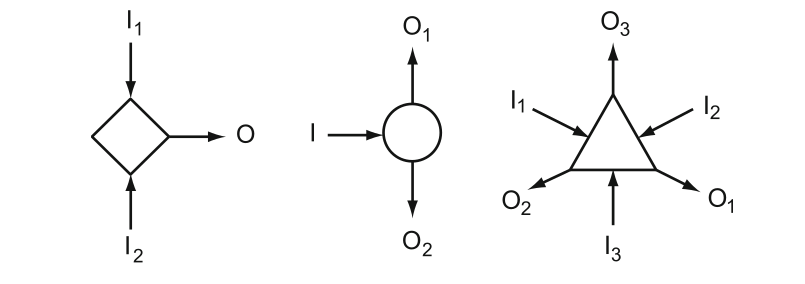
\includegraphics[width=9cm]{bilder/tokenBased.png}
       \caption{Merge, Fork und Tria}
       \label{fig:tokenBased}
\end{figure}    


Dabei führt Merge zwei Kabel zu einem zusammen, wobei die Tokens einfach 
nur weitergeleitet werden.
% 
Fork macht aus einem Token zwei.
%
Tria fügt zwei Tokens zusammen und je nach Eingabekabel kommt
die Ausgabe auf ein bestimmtes Kabel.
%
Für jedes Input Token  $ I_{i} \, (i \in \{1, 2, 3\}) $ und $ I_{j} \, (j \in 
\{1, 2, 3\}) $ erhalten wir das Ausgabe Token auf $O_{6-i-j}$.
%
Wobei das Zusammenführen beim Tria nur funktioniert wenn zwei Tokens da sind,
ein einzelnes Token wartet solange bis ein zweites kommt.
%
Diese Funktionalität in asynchronen Schaltkreisen hat die Aufgabe die 
verschiedenen nebenläufigen Berechnungen zu synchronisieren und entspricht
gewissermaßen dem Takt in synchronen Schaltkreises
und ist deshalb hervorzuheben.
%

%-----------------------------------------------------------------------------

\subsection{Token-pass Schaltkreise}
Der Name kommt von der Bauweise dieser Schaltkreise, sie verbinden einfach nur
Kabel miteinander durch die Tokens hindurchlaufen und die Schaltkreiselemente
geben diese weiter oder nicht. \\
%
Token-pass Schaltkreisen lassen die Zahl der Tokens gleich.
%
Tokens können nicht entstehen oder verschwinden und auch 
nicht auf andere Kabel wechseln.

\begin{figure}[h]
    \centering
    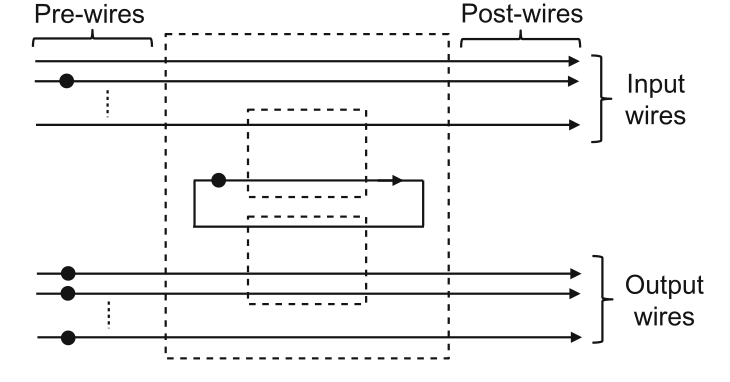
\includegraphics[width=8cm]{bilder/TokenPassScheme.png}
    \caption{Token-pass Schema}
    \label{fig:tokenPassScheme}
\end{figure} 


Token-pass Schaltkreise haben eine Menge an Eingabekablen die in
den Schaltkreis führen und eine Menge an Ausgabekabeln.
%
Wobei diese in einen Abschnit vor dem Schaltkreis (pre-wire) und einen Abschnit
danach (post-wire) eingeteilt werden.
%
Die Eingabekabel können im pre-wire Abschnitt beliebig Token haben die aber 
wenn vorhanden auch auf den post-wire Abschnitt geführt werden.
%
Die Ausgabekabel haben im pre-wire Abschnitt alle ein Token und haben dann
beliebig Tokens auf dem post-wire Abschnitt, entsprechend der Ausgabe.
%
Innerhalb des Schaltkreises können sich Schleifen befinden. 
%

%-----------------------------------------------------------------------------
\subsection{Von token-basiert nach token-pass}
%TODO text schreiben

\begin{figure}[h]
    \centering
    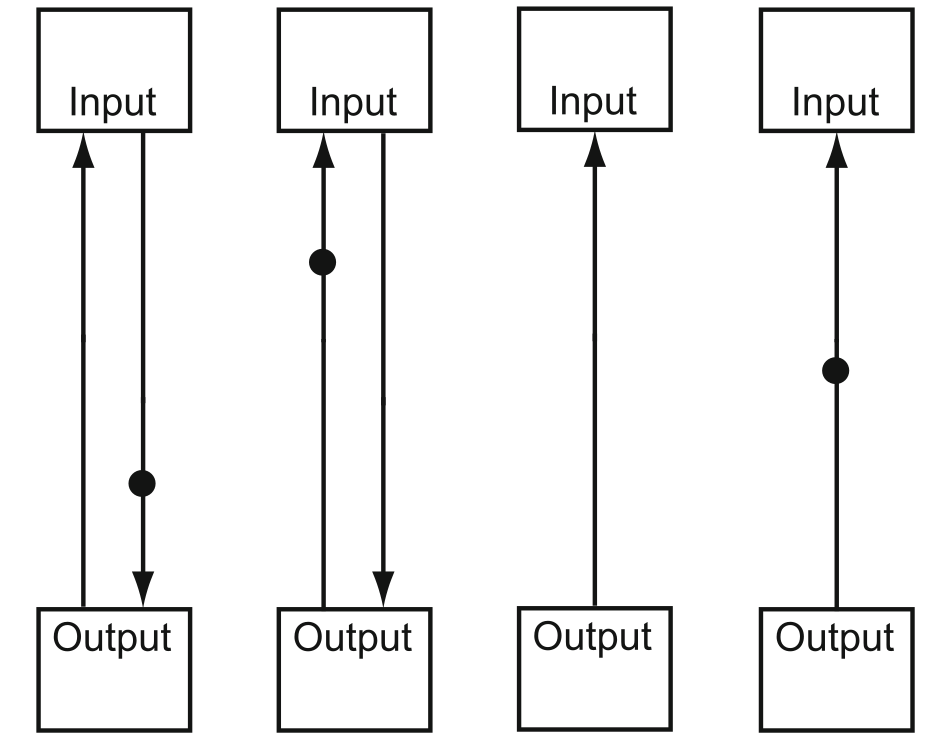
\includegraphics[width=7cm]{bilder/basedToPass.png}
    \caption{token-pass (links) und token-basiert (rechts)}
\end{figure}

Token-basierte Schaltkreise können äquivalent als token-pass Schaltkreise 
dargestellt werden, indem einfach aus jedem Kabel zwei werden und die Token 
sich entsprechend der Abbildung 3 verhalten.

%-----------------------------------------------------------------------------

\subsection{Brownsche Schaltkreise}
Brownsche Schaltkreise sind eine Erweiterung der token-pass Schaltkreise. 
%
Tokens können sich nun frei bewegen, angelehnt an die
brownsche Molekularbewegung.
%
Diese Fluktuation ist treibende Kraft für das Zusammenwirken der Tokens 
innerhalb der Schaltkreiselemente. 
%
Sie ermöglicht Tokens aus Sackgassen wieder zu entkommen,
was sich in einfacherem Design wiederspiegelt da nicht alles explizit 
modelliert werden muss.

%-----------------------------------------------------------------------------

\subsubsection{Polare token-pass brownsche Schaltkreise}
In polaren token-pass Schaltkreises existiert eine bevorzugte Richtung (Bias)
der Token, gekennzeichnet durch einen Pfeil.
%

\paragraph{Polares T-Element}
\begin{figure}[h]
    \centering
    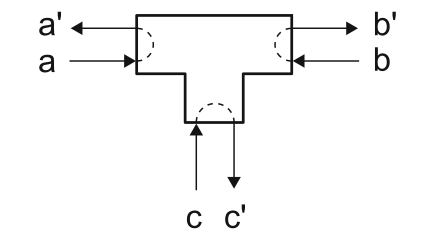
\includegraphics[width=7cm]{bilder/T_Element.png}
    \caption{T-Element}
    \label{fig:T_Element}
\end{figure}

Grundlegende Funktion des T-Elementes entspricht. 
%
Eingang c ist der Basis Eingang des T-Elementes, hier muss immer ein Token
anliegen damit es zur Verarbeitung kommt.
%
Wenn bei c ein Token anliegt und bei einem der beiden anderen
Eingänge a oder b auch ein Token anliegt werden diese vom T-Element 
entlang des gestrichelten Halbkreises auf das parallel verlaufende 
Kabel überführt.
%
Wenn bei a und b gleichtzeitig ein Token anliegt wird zufällig 
eines der beiden ausgewählt und mit c überführt.
 

%-----------------------------------------------------------------------------

\subsubsection{Nichtpolare token-pass brownsche Schaltkreise}
Die Tokens haben keinen Bias mehr und können frei fluktuieren.
%
Die nichtpolaren token-pass brownschen Schaltkreise haben eine neue Notation
an den Eingängen von T-Elementen (Kreise oder blank Symbole bzw. nichts).
%
Diese Notation macht Einschränkungen für die Funktion
der Kabel und des T-Elementes.
%
Wenn die Enden eines Kabels das gleiche Ende haben dann ist dieses Kabel nicht
polar. 
%
Wenn sie unterschiedlich sind entsprechen sie einem polaren Kabel, wobei 
der Bias dann in Richtung des Kreises vorliegt.
%
In einem T-Element können jetzt nur Eingänge miteinander verarbeitet werden
die das gleiche Symbol haben. \\
%
Ebenfalls neu sind die sogenannten Terminator Kabel, diese Kabel haben ein 
Kreissegment als Ende und halten einfach die Tokens 
davon ab das Kabel zu verlassen. \\
%
Für einige Kabel in einem nichtpolaren Schaltkreis ist ein Bias sinnvoll.
%
Ein Beispiel sind die Ausgabekabel da sich hier Tokens immer nur in eine 
Richtung bewegen sollten und nicht nach erfolgreicher Berechnung diese 
wieder rückwärtslaufen.
%
Die nicht-polaren Schaltkreise ermöglichen einfacheres Design und Verwendung
von weniger T-Elementen, weil bestimmtes Verhalten zum Verhindern von
Deadlocks, ausgelöst von Sackgassen, nicht expizit modelliert werden muss.

\begin{figure}[h]
    \centering
    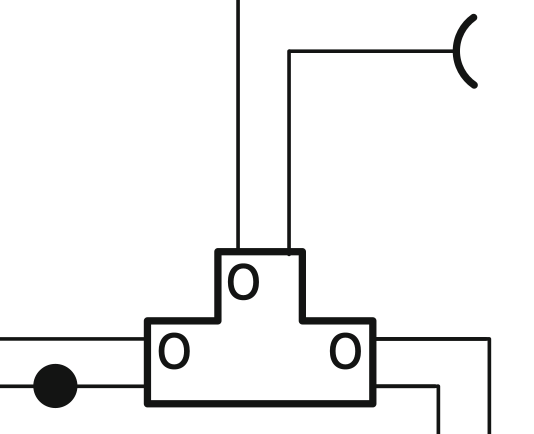
\includegraphics[width=5cm]{bilder/NonPolarTerminator.png}
    \caption{nichtpolares T-Element und Terminator Kabel}
    \label{fig:T_Element}
\end{figure}


%-----------------------------------------------------------------------------
%-----------------------------------------------------------------------------

\section{Universalität des T-Element}

In Abbildung 6 ist zu erkennen wie die token-basierten Schaltkreispirmitive 
(Merge, Fork und Tria) mit mithilfe des T-Elementes nachgebaut werden.
%
\\
Daraus folgt, dass das brownsche T-Element universell für die Klasse der 
token-pass brownschen Schaltkreise ist.
\\
%
Laut den Autoren ist dies sogar die Klasse aller berechenbarer Funktionen und
somit sind token-pass brownsche Schaltkreise berechnungsuniversell. 
%
Die Berechnungsuniversalität der token-basierten Schaltkreise wird in
\cite{Lee_2005} gezeigt, dies geschieht allerdings durch Verweisen auf 
noch ältere Aufsätze bis schließlich  auf \cite{Keller_1974} verwiesen wird.
%
Dadurch kann ich nicht nachvollziehen ob man wirklich von berechnungsuniversell
sprechen kann bzw. die Universalität von einer Implentierung erreicht
werden würde. 

\begin{figure}[h]
    \centering
    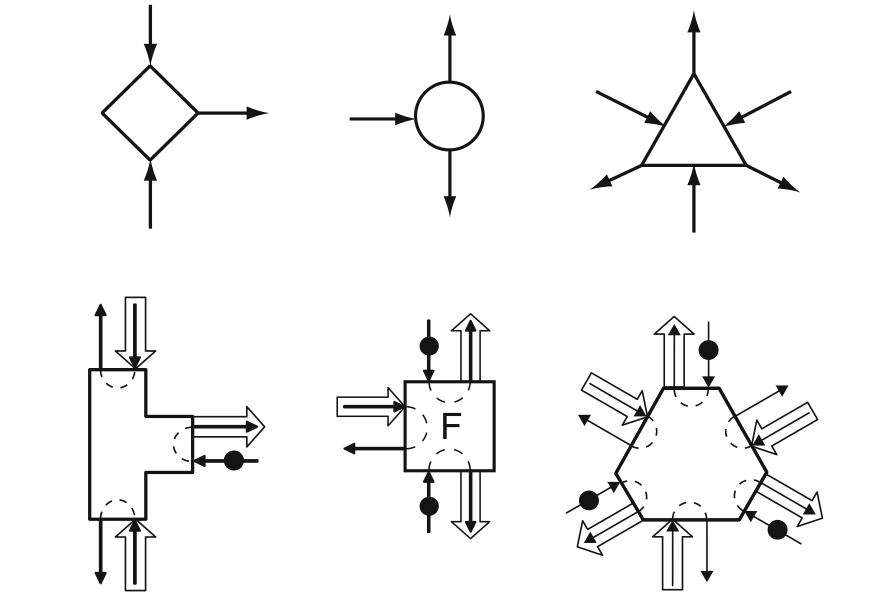
\includegraphics[width=7.5cm]{bilder/BasedToPass.png}
    \caption{Äquivalenz token-based und token-pass}
    \label{fig:BasedToPass}
\end{figure}


%\begin{figure}[h]
%    \begin{minipage}{0.45\textwidth}
%       \centering
%       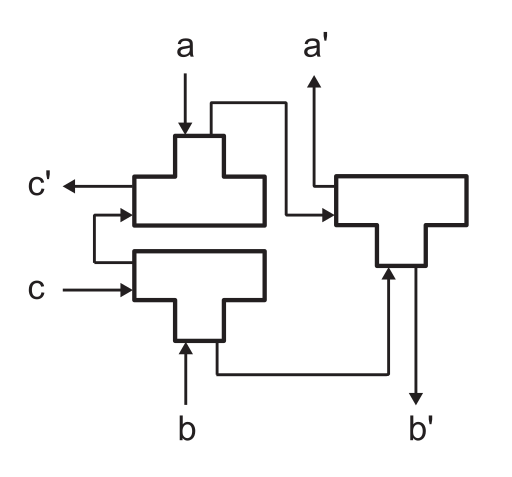
\includegraphics[width=6cm]{bilder/TP_Fork.png}
%       \caption{Fork aus T-Elementen}
%   \end{minipage}\hfill
%    \begin{minipage}{0.45\textwidth}
%       \centering
%       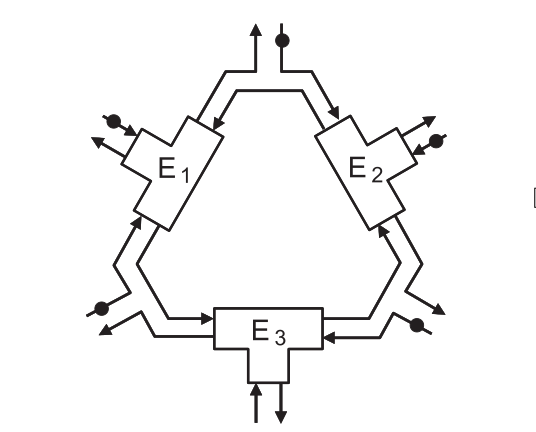
\includegraphics[width=6cm]{bilder/TP_Tria.png}
%       \caption{Tria aus T-Elementen}
%   \end{minipage}\hfill
%\end{figure}    

%
Das direkte Nachbauen von token-basierten Schaltkreisen mithilfe
der TP-Merge, TP-Fork und TP-Tria ist nicht effizient.
%
Da dabei das Fluktuierens der Tokens nicht ausgenutzt wird.
%
Beispielsweise benötigt ein 1-Bit Speicher der naiv mithilfe der 
Schaltkreisprimitiven nachgebaut ist insgesamt 26 T-Elemente.
%
Im nächsten Abschnitt werden wir sehen, dass dies sehr viel effizienter möglich
ist, wenn man Eigenschaften der brownschen token-pass Schaltkreise
beim Design richtig ausnutzt.


%-----------------------------------------------------------------------------
%-----------------------------------------------------------------------------

\section{1-Bit Speicher}
Nun soll anhand eines 1-Bit Speichers die Funktionsweise von brownschen 
token-pass Schaltkreisen erläutert werden.
%
Mithilfe von polaren T-Elementen ist es möglich einen 1-Bit Speicher mit 8
T-Elementen zu bauen \cite{Peper_Fundamentals_2013}. 
%
Bei nicht-polaren brownschen T-Elementen sind es sogar
nur 7  T-Elemente \cite{Peper_nonPolar_2018}.

\begin{figure}[h]
      \centering
      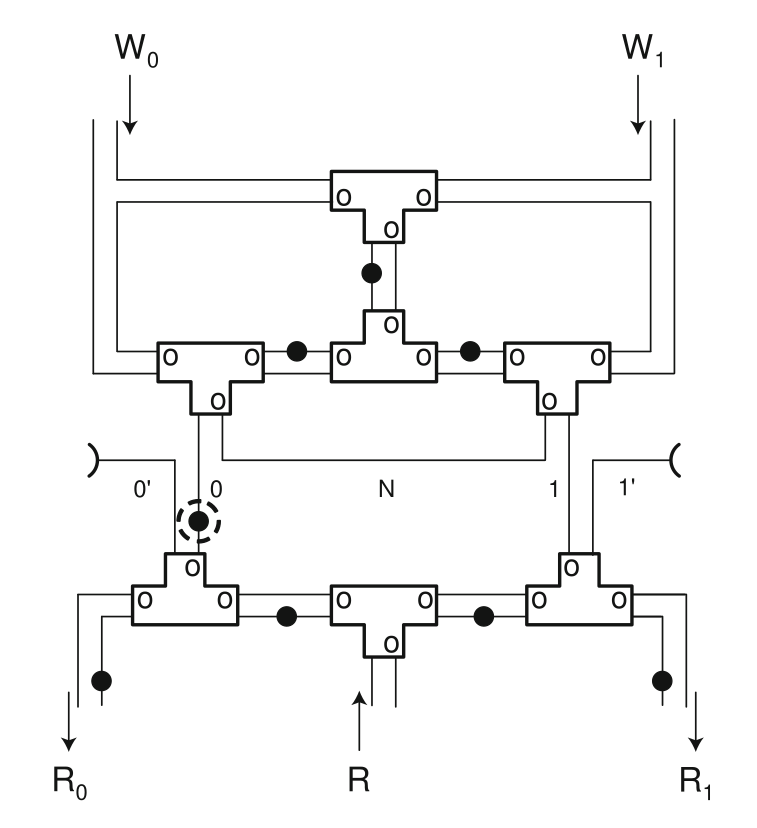
\includegraphics[width=9cm]{bilder/NonPolarMemory.png} 
      \caption{1-Bit Speicher nicht polar token pass}
\end{figure}

Grundlegend gibt es jeweils eine Menge an T-Elementen für das Lesen bzw. 
Schreiben.
%
Von zentraler Bedeutung ist ein Token in der Mitte des Schaltkreises, das über 
seine Position den derzeitigen Zustand des Speichers angibt.
%
Der Speicher soll mit einer 0 initialisiert sein.
%
Entsprechend ist auch das mittlere Token (umkreist) in Abbildung 7 positioniert.


\subsection{Schreibvorgang}
Zunächst soll der Schreibvorgang erläutert werden.
%
Wobei eine 0 gespeichert ist und eine 1 geschrieben wird.
%
Der Schaltkreis durchläuft 6 verschieden Zustände, wobei einer 
davon eine Sackgasse ist.
%
In Abbildung 8 sind die entsprechenden Übergänge gekennzeichnet 
und jeweils das T-Element was als letztes Tokens bewegt hat grau markiert.

\begin{figure}[h]
      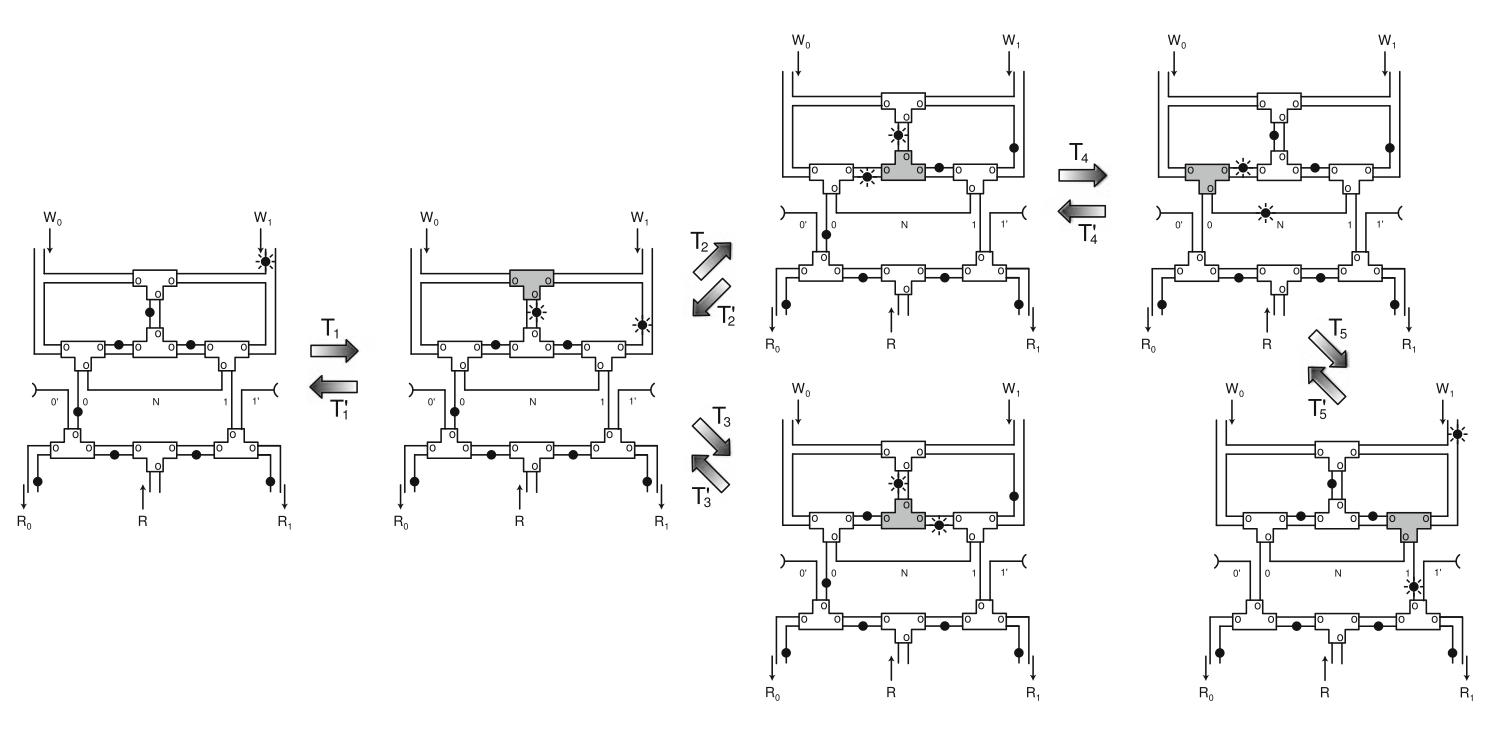
\includegraphics[width=14cm]{bilder/write1Mem.png} 
      \caption{Schreiben einer 1}
\end{figure}

\subsection{Lesevorgang}
Jetzt wird das Auslesen der geschriebenen 1 erläutert.

\begin{figure}[h]
      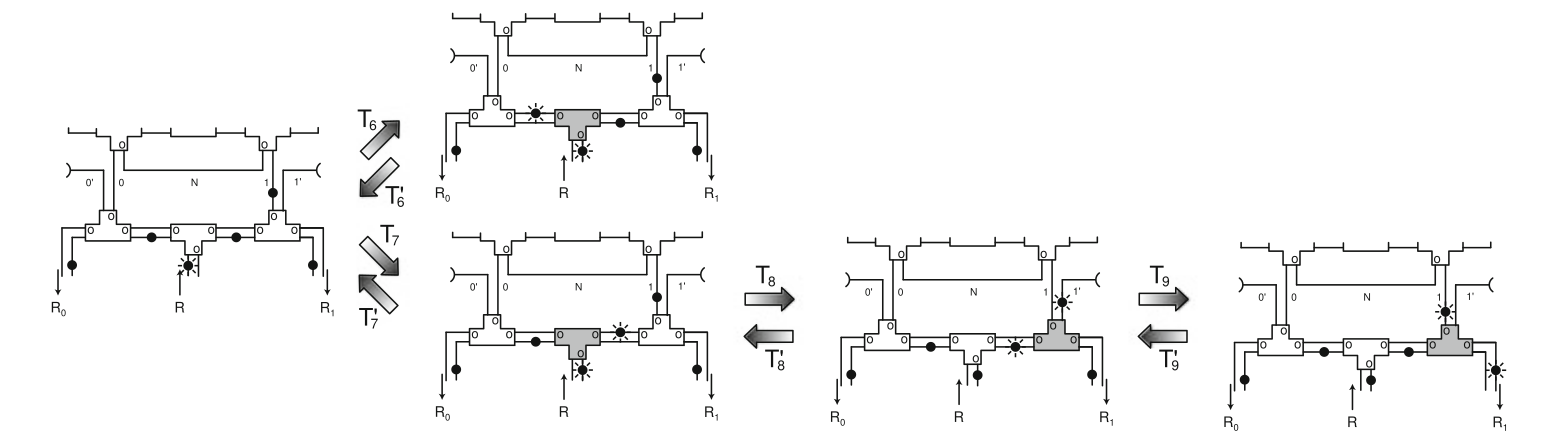
\includegraphics[width=14cm]{bilder/read1Mem.png} 
      \caption{Lesen einer 1}
\end{figure}


%-----------------------------------------------------------------------------
%-----------------------------------------------------------------------------

\section{UND-Bauteil}

\begin{figure}[h]
    \centering
    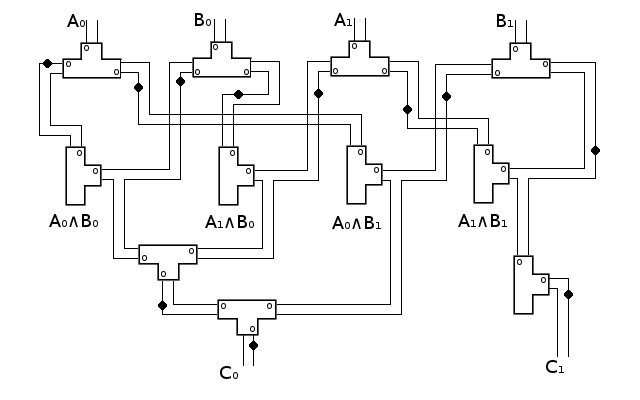
\includegraphics[width=12cm]{bilder/UndUnd.png}
    \caption{UND-Gatter aus 11 T-Elementen}
\end{figure}    

Als Teil meiner Eigenarbeit im Rahmen dieses Proseminars habe ich ein UND-Gatter
mithilfe von nicht-polaren T-Elementen entworfen. \\
%
Es benutzt den Suchmechanismus der Tokens und Backtracking falls sie in eine 
Sackgasse laufen. 
%
Die Idee ist jede mögliche Eingabekombination jeweils mit einem 
logischen UND zu verknüpfen. 
%
Das erste T-Element jeder Eingabe wird zum Modellieren
der möglichen zwei Wege benutzt.
%
Die beiden Eingabe Token versuchen sich in dem der Eingabe entsprechenden
T-Element, welches dem UND entspricht, zu finden.
%
Haben sich beide Input Tokens gefunden wird ein Token weitergeleitet.
Bei der Eingabe $ (A_{1},\, B_{1}) $ wird dieses Token direkt zu Ausgabe
$ C_{1} $, bei allen anderen Eingabemöglichkeiten werden die Token mithilfe
von zwei weiteren T-Elementen zur Ausgabe $ C_{0} $ zusammengeführt. 

%-----------------------------------------------------------------------------

\subsection{Initialisierung}
Es ist eine Initialisierung auf der Abbildung gegeben (die Position der Tokens), 
außerdem sind die Kreise in den T-Elementen für eine korrekte Berechnung
elementar.
%
Diese Initialisierung ist nicht eindeutig und auch die Anordnung der
Elemente ist veränderbar, was im Hinblick auf möglichst kurze Kabel 
für eine schnellere Berechnung von Interesse ist.

%-----------------------------------------------------------------------------

\subsection{Korrektheit}
Eine interessante Frage ist nun ob die Korrektheit dieses Schaltkreises
beweisbar ist. Wenn wir die angegebene Initialisierung vorraussetzen können,
können wir uns die Korrektheit schnell klar machen indem :


%-----------------------------------------------------------------------------
%-----------------------------------------------------------------------------

\section{Zusammenfassung und Ausblick}
In dem Aufsatz \cite{Peper_nonPolar_2018} wird eine neue Art
von Schaltkreis vorgestellt der zukünfitig in der Nanoelektronik eingesetzt
werden könnte.
%
Aufbauend auf den polaren brownschen token pass Schaltkreisen aus 
\cite{Peper_Fundamentals_2013} werden nicht polare Kabel und T-Elemente 
eingeführt deren Token keinen Bias in ein Richtung haben. 
%
Dabei ist das Konzept von brownscher Bewegung der Signale (Tokens) 
der interessante und neue Aspekt der es ermöglicht neue Arten von Schaltkreisen 
zu designen und auf ihre Eigenschaften zu untersuchen.
%
Jedoch sind Dinge wie Geschwindigkeit der Berechnung, Korrektheit beweisen und 
welche arten von konkreten Implementierungen möglich sind noch zu klären.

%-----------------------------------------------------------------------------

\subsection{Geschwindigkeit der Berechnung}
Die Fluktoation der Tokens auf einem Kabel der Länge L führt zu 
erwartet Zeit O(L²).
%
Desweiteren kann man Sperren einsetzen, sodass Tokens
auf bestimmten Kabeln sich nur in eine Richtung bewegen können. 
%
Dies ist auf den Ausgabekabeln sinnvoll.

%-----------------------------------------------------------------------------

\subsection{Korrektheit}
Zwar sind mit nichtpolaren brownschen Schaltkreisen Schaltkreiselemente mit
weniger Bauteilen möglichen.

%
Allerdings ist das Vorgehen beim Entwerfen und Überprüfen dieser Art von 
Schaltkreisen auf Korrektheit noch unklar. 

%-----------------------------------------------------------------------------

\subsection{Implementierung}
Das T-Element ist geeignet um theoretisch dieses Berechnungsmodell zu 
untersuchen ist jedoch für eine Implementierung nicht optmial.
%
Es hat zu viele Kabel und ist zu komplex um sinnvoll als Schaltkreisprimitv
eingesetzt zu werden. 
%
Allerdings ist es für simplere Schaltkreiselemente nicht möglich in auch ohne 
Fluktuation zu funktionieren.
%
Auch kann es zu Interaktionen zwischen Tokens kommen die von bei diesem Modell
nicht beachtet werden. (z.B. Elektronen als Tokens und entsprechende 
Elektromagnetische Felder)
%
Auch kann es zu Interaktionen zwischen Tokens kommen die von bei diesem Modell
nicht beachtet werden. (z.B. Elektronen als Tokens und entsprechende 
Elektromagnetische Felder). Desweiteren sind Dinge wie Token bleiben nur
auf einem Kabel nicht unbedingt leicht um zu setzen für die Implementierung.



% Literaturverzeichnis erstellen 
\bibliographystyle{plain}
\bibliography{\jobname}

\end{document}
